\begin{frame}{Line graphs}%time sets are not equal
			\begin{columns}[T]
				\column{.5\textwidth}
					\only<1>{\begin{block}{pH}
						\begin{itemize}
							\item Class 2 always contains the lowest pH mean instead of 6
							\item Class 3 belongs between 5 and 6
						\end{itemize}
					\end{block}}
					\only<2>{\begin{block}{ANC $\mu eqL^{-1}$}
						\begin{itemize}
							\item All classes decrease from set 2 to 3 except for class 2, which is increasing
							\item Concentrations vary greatly across classes, classes 1 and 2 are more than double the others
							\item They are the lowest in class 2 which corresponds to the low pH values for class 2, but class 2 is also the only class that is increasing
						\end{itemize}
					\end{block}}
					\only<3>{\begin{block}{Nitrate $\mu eqL^{-1}$}		
						\begin{itemize}
							\item The odd classes all have decreasing means from sets 2 to 3
							\item Classes 2 and 4 have mean values for set 3 that are greater than set 2, but the rate of change is decreasing
							\item Class 6 is always increasing
							%\item The odd classes all have decreasing negative trends from set 2 to 3 while classes 2 and 4 have decreasing positive trends between 2 and 3
						\end{itemize}
					\end{block}}
					\only<4>{\begin{block}{Sulfate $\mu eqL^{-1}$}
						\begin{itemize}
							\item Set 3 means are greater than set 2 means in all but class 2
							\item In classes 1, 4, and 6 the rate of change is decreasing
							\item Concentrations seem to be increasing across the sets in classes 3 and 5
							\item Class 2 has a decreasing decreasing trend
						\end{itemize}
					\end{block}}
				\column{.25\textwidth}
					\centering \tiny \textbf{Class 1}
					\begin{figure}\centering \pgfplotsset {try min ticks=3}
           						\begin{tikzpicture}
								\begin{axis}[scale=.225,xtick = {1,2,3},tick label style={font=\tiny},scale mode= stretch to fill, ytick=data]
									\only<1>{\addplot coordinates{(1,6.57) (2,6.65) (3,6.77)};}
									\only<2>{\addplot coordinates{(1,149.76) (2,173.07) (3,165.56)};}
									\only<3>{\addplot coordinates{(1,12.03733) (2,16.77264) (3,16.28445)};}
									\only<4>{\addplot coordinates{(1,36.09) (2,39.23) (3,39.70)};}
								\end{axis}
							\end{tikzpicture}
          					\end{figure}
					\textbf{Class 2}
					\begin{figure}\centering \pgfplotsset{try min ticks=3}						
           						\begin{tikzpicture}
								\begin{axis}[scale=.225,xtick = {1,2,3},tick label style={font=\tiny},scale mode= stretch to fill, ytick=data]
									\only<1>{\addplot coordinates{(1,6.25) (2,6.32) (3,6.47)};}
									\only<2>{\addplot coordinates{(1,40.75) (2,42.20) (3,44.45)};}
									\only<3>{\addplot coordinates{(1,26.61657) (2,29.20006) (3,30.07626)};}
									\only<4>{\addplot coordinates{(1,51.68) (2,48.19) (3,47.41)};}
								\end{axis}
							\end{tikzpicture}
          					\end{figure}
					\textbf{Class 3}
					\begin{figure}\centering \pgfplotsset{try min ticks=3}
           						\begin{tikzpicture}
								\begin{axis}[scale=.225,xtick = {1,2,3},tick label style={font=\tiny},scale mode= stretch to fill, ytick=data]
									\only<1>{\addplot coordinates{(1,6.45) (2,6.55) (3,6.68)};}
									\only<2>{\addplot coordinates{(1,170.03) (2,172.82) (3,161.81)};}
									\only<3>{\addplot coordinates{(1,25.97658) (2,27.68893) (3,26.17686)};}
									\only<4>{\addplot coordinates{(1,53.98) (2,54.25) (3,58.22)};}
								\end{axis}
							\end{tikzpicture}
          					\end{figure}
				\column{.25\textwidth}
					 \centering \tiny \textbf{Class 4}
					\begin{figure}\centering \pgfplotsset{try min ticks=3}
           						\begin{tikzpicture}
								\begin{axis}[scale=.225,xtick = {1,2,3},tick label style={font=\tiny},scale mode=stretch to fill, ytick=data]
									\only<1>{\addplot coordinates{(1,6.50) (2,6.58) (3,6.68)};}
									\only<2>{\addplot coordinates{(1,75.52) (2,69.90) (3,64.13)};}
									\only<3>{\addplot coordinates{(1,12.55250) (2,17.50807) (3,18.71509)};}
									\only<4>{\addplot coordinates{(1,25.53) (2,29.04) (3,29.33)};}
								\end{axis}
							\end{tikzpicture}
          					\end{figure}
					\textbf{Class 5}
					\begin{figure}\centering \pgfplotsset{try min ticks=3}
           						\begin{tikzpicture}
								\begin{axis}[scale=.225,xtick = {1,2,3},tick label style={font=\tiny},scale mode= stretch to fill, ytick=data]
									\only<1>{\addplot coordinates{(1,6.50) (2,6.50) (3,6.77)};}
									\only<2>{\addplot coordinates{(1,76.96) (2,77.84) (3,73.55)};}
									\only<3>{\addplot coordinates{(1,4.35218) (2,7.43691) (3,6.44408)};}
									\only<4>{\addplot coordinates{(1,27.11) (2,30.43) (3,36.16)};}
								\end{axis}
							\end{tikzpicture}
          					\end{figure}
					\textbf{Class 6}
					\begin{figure}\centering \pgfplotsset{try min ticks=3}
           						\begin{tikzpicture}
								\begin{axis}[scale=.225,xtick = {1,2,3},tick label style={font=\tiny},scale mode= stretch to fill, ytick=data]
									\only<1>{\addplot coordinates{(1,6.41) (2,6.44) (3,6.52)};}
									\only<2>{\addplot coordinates{(1,68.01) (2,55.68) (3,46.80)};}
									\only<3>{\addplot coordinates{(1,21.13072) (2,24.87664) (3,31.77411)};}
									\only<4>{\addplot coordinates{(1,28.35) (2,34.31) (3,36.86)};}
								\end{axis}
							\end{tikzpicture}
          					\end{figure}
			\end{columns}
		\end{frame}